\section{Traceability Architektur-Varianten}
\label{sec:traceability-architecture}

% \hl{structure notes start}
% \begin{itemize}
%     \item Basismodell / Subset vom Metamodell beschreiben auf welchen die Traceability Architektur aufbaut
%     \item Pro Architektur ein Kapitel, welche die Funktionsweise beschreibt und wie es gedenkt die Anforderungen zu erfüllen
% \end{itemize}
% \hl{structure notes end}

\subsection{Variante 1: Control-centric Bundling}
\label{sec:trace-arch-variant1}

\textbf{Ansatz}: Für jede Control in der jeweiligen Verordnung wird ein Mapping zu einem Plattform-Bundle gemacht. Also eine Control beinhaltet Plattform-Policies X, Y und Z. Beim Deployment einer \ac{lz} wählt das Blueprint aus welche Controls benötigt werden (z.B. keine Profile, erhöhter Schutzbedarf, etc.)

\textbf{Fokus}: Traceability

\textbf{Pros}
\begin{itemize}
    \item Rückverfolgbarkeit ist trivial: Das Ergebnis des Enforcements wird direkt einer Control-ID zugeordnet.
    \item Ideal für Audits (\flqq Zeig mir alle implementierten Controls\frqq).
\end{itemize}

\textbf{Cons}
\begin{itemize}
    \item Viele kleine Artefakte → erfordern Automatisierung und eine Build-Pipeline
    \item Einige Provider bevorzugen grössere Sets
\end{itemize}

\textbf{Fazit}: Diese Variante ist diejenige welche am besten die Traceability Anforderungen erfüllt, aber auch die aufwändigste in der Umsetzung ist. Es könnte als \flqq Goldstandard\frqq\ für die Traceability Architektur angesehen werden, aber es muss evaluiert werden ob der Aufwand gerechtfertigt ist im Vergleich zu den anderen Varianten.

\begin{figure}[H]
    \centering
    
\includegraphics[width=\textwidth]{ip6-ideation-Traceability-Architecture-control-centric.drawio.pdf}
    \caption{Control-centric Traceability Architektur Variante}
    \label{fig:traceability-architecture-control-centric}
\end{figure}

\subsection{Variante 2: LZ component-centric Bundling}
\label{sec:trace-arch-variant2}

\textbf{Ansatz}: Die Controls werden nach \ac{lz}-Komponenten in Komponenten-Profiles gebündelt. Diese Profiles werden den Plattformrichtlinien zugeordnet. Bei der Bereitstellung einer \ac{lz} wählt der Blueprint die benötigten Komponenten und die Profiles der einzelnen Komponenten aus.

\textbf{Fokus}: Engineering, Verteilung an Expertengruppen/Teams, aber mit Rückverfolgbarkeit

Eine Regulation bildet ein Regelwerk wie z.B. \ac{si001} ab, welches die verschiedenen Controls enthält. Eine Control ist je eine Anforderung welche eingehalten werden muss damit die Control als eingehalten gilt.

\textbf{Funktionsweise}: Die Controls haben mind. eine Beziehung zu mind. einer \ac{lz}-Komponente, welche die Control implementiert. Für jede \ac{lz}-Komponente existieren verschiedene Profiles, diese Profiles bauen aufeinander auf, heisst die Nächsthöhere enthält Vorherige auch. Ein Profile kann jeweils mehrere Controls implementieren und bildet das Mapping zwischen Controls und konkreten Policies auf der jeweiligen Zielplattform. Policies können sowohl selbst definiert als auch vom Provider bereitgestellt sein.

\begin{figure}[H]
    \centering
    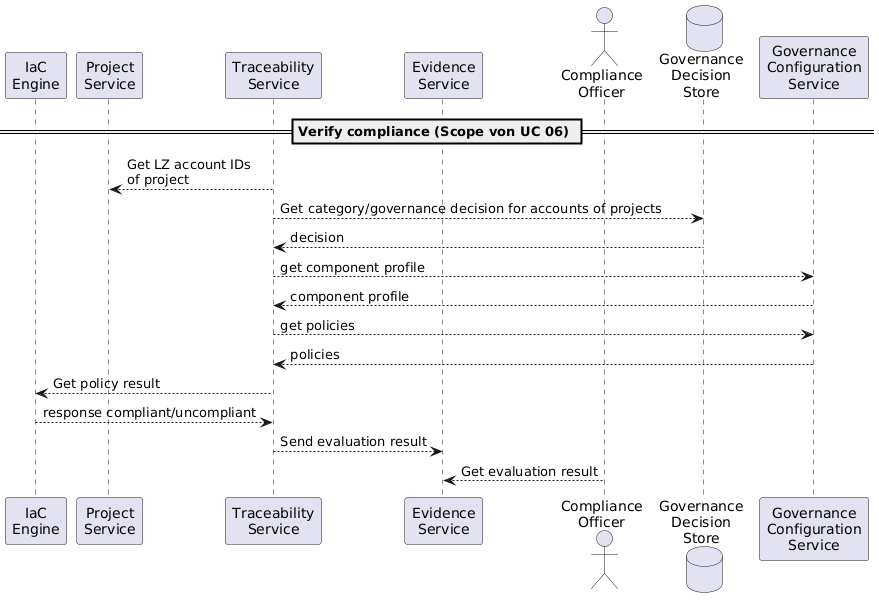
\includegraphics[width=\textwidth]{graphics/sequence-diagramm-poc_variant2_verify-compliance.png}
    \caption{Sequenz-Diagramm für Verifikation der Compliance nach Traceability Architektur Variante 2}
    \label{fig:methodology-poc-variant2-sequence-verification}
\end{figure}

\textbf{Pros}
\begin{itemize}
    \item Passt zur Implementierungspraxis von Teams: Netzwerkrichtlinien werden gemeinsam verwaltet
    \item Weniger Bundles, einfachere Einführung
\end{itemize}

\textbf{Cons}
\begin{itemize}
    \item Die Rückverfolgbarkeit erfordert einen zusätzlichen Suchschritt: \flqq Richtlinie X befindet sich im Bundle Netzwerk → enthält Controls A, B, C\frqq
    \item Einige Policies implementieren mehrere Controls (1:n)
\end{itemize}

\textbf{Fazit}: Diese Variante bietet einen guten Kompromiss zwischen Rückverfolgbarkeit und Praktikabilität, da sie die Implementierungspraxis der Teams berücksichtigt, aber dennoch eine gewisse Rückverfolgbarkeit ermöglicht. Es könnte als \flqq Silberstandard\frqq\ für die Traceability Architektur angesehen werden, da es eine praktikable Lösung darstellt, ohne den Aufwand der Control-zentrierten Variante zu erfordern.

\begin{figure}[H]
    \centering
    
\includegraphics[width=\textwidth]{ip6-ideation-Traceability-Architecture-component-centric.drawio.pdf}
    \caption{Component-centric Traceability Architektur Variante}
    \label{fig:traceability-architecture-component-centric}
\end{figure}

\subsection{Variante 3: LZ category centric Bundling}
\label{sec:trace-arch-variant3}

\textbf{Ansatz}: Controls werden nach Profiles gebündelt, welche die Rules für alle Komponenten enthalten. Diese Profiles umfassen die entsprechenden Policies. Beim deployen einer \ac{lz} wählt der Blueprint nur die \ac{lz}-Profiles aus, der Rest wird abstrahiert.

\textbf{Fokus}: LZ-Kategorien mit Vereinfachung für den Endnutzer, da die Profile alles umfasst, ohne dass viel ausgewählt werden muss.

\textbf{Detailbeschreibung}: In dieser Architektur-Variante werden die Controls in Profiles gebündelt, die alle relevanten Regeln für die verschiedenen Komponenten enthalten. Jede Profile repräsentiert eine bestimmte \ac{lz}-Kategorie, die eine Risikoklasse oder einen Anwendungsfall abdeckt. Beim Deployen einer \ac{lz} wählt das Blueprint einfach die entsprechende Profile aus, ohne dass der Benutzer sich mit den einzelnen Controls oder Policies auseinandersetzen muss. Diese Herangehensweise bietet eine extrem einfache Anwendung und eine klare Customer Story, da die Kategorien direkt mit den Risikoklassen verknüpft sind. Allerdings führt dies zu einer hohen Duplikation von Controls über verschiedene Kategorien hinweg, und die Rückverfolgbarkeit zu einzelnen Controls erfordert die Pflege eines Manifests, das auflistet, welche Controls in welcher Profile enthalten sind.

\textbf{Pros}
\begin{itemize}
    \item Extrem einfache Anwendung (\flqq regulierte Profile anwenden\frqq)
    \item Klare Customer Story: Kategorien repräsentieren Risikoklassen
\end{itemize}

\textbf{Cons}
\begin{itemize}
    \item Hohe Duplikation von Controls über Kategorien hinweg
    \item Rückverfolgbarkeit zu einzelnen Controls ist gegeben, aber man muss ein Manifest \flqq Controls in der Profile\frqq\ führen
\end{itemize}

\textbf{Fazit}: Diese Variante bietet die einfachste Anwendung für den Endnutzer, da sie die Komplexität der Auswahl von Controls und Policies abstrahiert. Es könnte als \flqq Bronze-Standard\frqq\ für die Traceability Architektur angesehen werden, da es eine benutzerfreundliche Lösung darstellt, aber mit erheblichen Nachteilen in Bezug auf Duplikation und Rückverfolgbarkeit einhergeht.

\begin{figure}[H]
    \centering
    
\includegraphics[width=\textwidth]{ip6-ideation-Traceability-Architecture-category-centric.drawio.pdf}
    \caption{LZ Category centric Traceability Architektur Variante}
    \label{fig:traceability-architecture-category-centric}
\end{figure}

\subsection{Variante 4: LZ Provider-native Bundling}
\label{sec:trace-arch-variant4}

\textbf{Ansatz}: Controls werden direkt durch die native Policy-Abstraction des Providers dargestellt (Azure Initiatives, AWS SCP usw.). Diese werden direkt auf die Komponenten angewendet.

\textbf{Fokus}: Die Anwendung von Richtlinien auf Ressourcen, weniger auf die Nachvollziehbarkeit (à la MVP). Initiativen/Bundles existieren bereits von verschiedenen Cloud-Providern.

\textbf{Detailbeschreibung}: In dieser Architektur-Variante werden die Controls direkt durch die nativen Richtlinienabstraktionen der Cloud-Provider dargestellt. Das bedeutet, dass die Implementierung der Controls direkt auf den Ressourcen erfolgt, ohne dass eine zusätzliche Abstraktionsschicht wie Bundles oder Profiles erforderlich ist. Diese Herangehensweise ermöglicht eine optimale Leistung und eine enge Ausrichtung an den Mechanismen der Provider, da sie die nativen Funktionen und Tools nutzt. Allerdings führt dies zu einer schlechteren Vergleichbarkeit über verschiedene Cloud-Provider hinweg, da jeder Provider unterschiedliche Formate und Strukturen für seine Richtlinien hat. Die Rückverfolgbarkeit erfordert daher eine Normalisierung über die verschiedenen Evidenceformate der Provider hinweg, um sicherzustellen, dass die Controls konsistent identifiziert und verfolgt werden können.

\textbf{Fazit}: Diese Variante bietet die beste Leistung und Providerausrichtung, da sie die nativen Mechanismen der Cloud-Provider nutzt. Es könnte als \flqq Performance-Standard\frqq\ für die Traceability Architektur angesehen werden, da sie die effizienteste Nutzung der Ressourcen ermöglicht, aber mit erheblichen Herausforderungen in Bezug auf Vergleichbarkeit und Rückverfolgbarkeit einhergeht.

\textbf{Pros}
\begin{itemize}
    \item Operativ sauber: Nutzung der nativen Mechanismen der Provider
    \item Beste Leistung und Providerausrichtung
\end{itemize}

\textbf{Cons}
\begin{itemize}
    \item Cloud-übergreifende Vergleichbarkeit wird schlechter
    \item Traceability muss über verschiedene Evidenceformate der Provider hinweg normalisiert werden
\end{itemize}

\begin{figure}[H]
    \centering
    
\includegraphics[width=\textwidth]{ip6-ideation-Traceability-Architecture-provider-native.drawio.pdf}
    \caption{LZ Provider Native Traceability Architektur Variante}
    \label{fig:traceability-architecture-provider-native}
\end{figure}